% Chapter 1

\chapter{Introducción general} % Main chapter title
\label{Chapter1} % For referencing the chapter elsewhere, use \ref{Chapter1}
\label{IntroGeneral}

%----------------------------------------------------------------------------------------

% Define some commands to keep the formatting separated from the content
\newcommand{\keyword}[1]{\textbf{#1}}
\newcommand{\tabhead}[1]{\textbf{#1}}
\newcommand{\code}[1]{\texttt{#1}}
\newcommand{\file}[1]{\texttt{\bfseries#1}}
\newcommand{\option}[1]{\texttt{\itshape#1}}
\newcommand{\grados}{$^{\circ}$}

%----------------------------------------------------------------------------------------
En este capítulo se presentan conceptos básicos sobre las tecnologías y técnicas que fueron utilizadas en el desarrollo del trabajo. Se abordan nociones sobre inteligencia artificial, aprendizaje automático, aprendizaje profundo, redes neuronales convolucionales, visión artificial y servicios en la nube. También se citan trabajos anteriores que inspiraron a este, las motivaciones para llevarlo a cabo junto a sus objetivos y alcances.

%----------------------------------------------------------------------------------------
\section{Inteligencia artificial, aprendizaje automático y aprendizaje profundo}

Inteligencia artificial (AI, \textit{Artificial Intelligence}), aprendizaje automático (ML, \textit{Machine Learning}) y aprendizaje profundo (DL, \textit{Deep Learning}), son términos muy utilizados hoy en día en el mundo del desarrollo tecnológico \cite{ai_ml_dl}. Aunque estos términos son muy parecidos, entre ellos existen dependencias que pueden ser visualizadas con ayuda de la figura \ref{fig:ai_ml_dl}.

\begin{figure}[h]
	\centering
	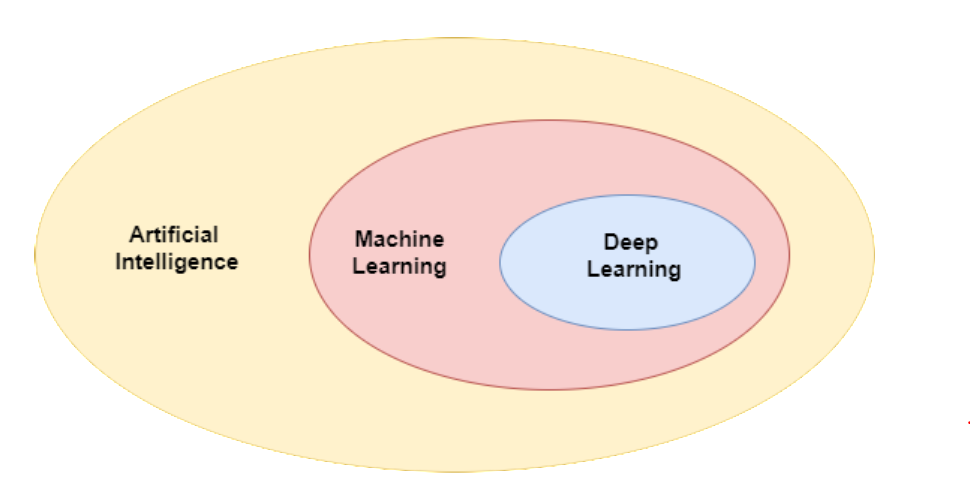
\includegraphics[scale=0.25]{./Figures/ai_ml_dl.png}
	\caption{Diferencias entre AI, ML y DL.}
	\label{fig:ai_ml_dl}
\end{figure}

\subsection{Inteligencia artificial}
Es un área de la computación que permite a los sistemas computacionales imitar la inteligencia humana para entender su entorno y tomar acciones que maximicen sus posibilidades de lograr sus objetivos \cite{ai_def}. Sus aplicaciones más importantes se encuentran en las áreas de comercio, educación, robótica, salud, agricultura, automotriz y finanzas\cite{ai_apps}. Todos los sistemas de inteligencia artificial reales e hipotéticos pueden ser clasificados en alguno de los siguientes tipos \cite{ai_types}:
\begin{itemize}
	\item Inteligencia artificial estrecha: también conocida como inteligencia artificial débil, su objetivo es llevar a cabo un solo tipo de tarea. Estos sistemas no poseen conciencia y no son manejados por sentimientos como lo haría un humano. Algunos ejemplos son los \textit{chatbots} o los automóviles autónomos.
	\item Inteligencia artificial general: también conocida como inteligencia artificial fuerte, es un concepto en el que las máquinas exhiben inteligencia humana. Estos sistemas tendrían la capacidad de aprender, entender y actuar de tal manera que sería indistinguible a un humano. Actualmente no existe, pero es utilizado conceptualmente en industrias como el cine.
	\item Super inteligencia artificial: también forma parte de la inteligencia artificial fuerte. Se le considera muy poderosa por ser capaz de volverse consciente y autónoma. No solo replica el comportamiento humano, sino que lo supera. Puede pensar mejor y tener más habilidades. Sin embargo, esta tecnología aún está en desarrollo.
\end{itemize}

\subsection{Aprendizaje automático}
Es un subconjunto de AI que utiliza algoritmos de aprendizaje estadísticos para construir sistemas con la habilidad de aprender automáticamente y mejorar a partir de experiencias previas sin ser explícitamente programados para esto \cite{ml_def}. Muchos de los servicios de recomendación empleados por empresas como Netflix, YouTube o Spotify, utilizan ML para adaptarse a un usuario en particular y ofrecer una mejor experiencia más personalizada \cite{ml_apps}. Estos algoritmos pueden ser clasificados de la siguiente manera \cite{ml_types}
\begin{itemize}
	\item Aprendizaje supervisado: se refiere al aprendizaje modelos a partir de un conjunto de datos, mejor conocidos como \textit{dataset}, cuyas respuestas son conocidas con antelación y están asociadas a una etiqueta o \textit{label}. Por ejemplo, el \textit{dataset} pueden ser muchas fotografías de gatos y el \textit{label} asociado el nombre de este animal. De esta manera el modelo es entrenado para generar predicciones de datos nuevos.
	
	\item Aprendizaje no supervisado: es usado cuando los datos utilizados para el aprendizaje no tienen \textit{labels}. Su objetivo principal es aprender acerca de los datos e inferir patrones sin ningún tipo de referencia sobre las respuestas esperadas. Es mayormente empleado como parte del análisis exploratorio de datos \cite{ai_ml_dl}.
	
	\item Aprendizaje reforzado: es el aprendizaje mediante la interacción continua con el entorno con el método de prueba y error, y utiliza continuamente la retroalimentación de sus acciones y experiencias previas. Este tipo de aprendizaje emplea recompensas si se realizan acciones correctas y penalizaciones si son incorrectas.
\end{itemize}

\subsection{Aprendizaje profundo}
Es una técnica de ML que está inspirada en la forma en la que el cerebro humano filtra información \cite{dl_def}. Cómo DL procesa información de manera similar al cerebro humano, sus aplicaciones son tareas que un humano generalmente realiza, como distinguir entre un peatón o un poste de luz en el caso de automóviles autónomos. El componente principal de DL son las redes neuronales artificiales, que son capas de nodos interconectados, donde existe una capa de entrada, una o varias capas ocultas y una capa de salida. En la figura \ref{fig:dl_nn} se puede observar la arquitectura de una red neuronal artificial.
\begin{figure}[h]
	\centering
	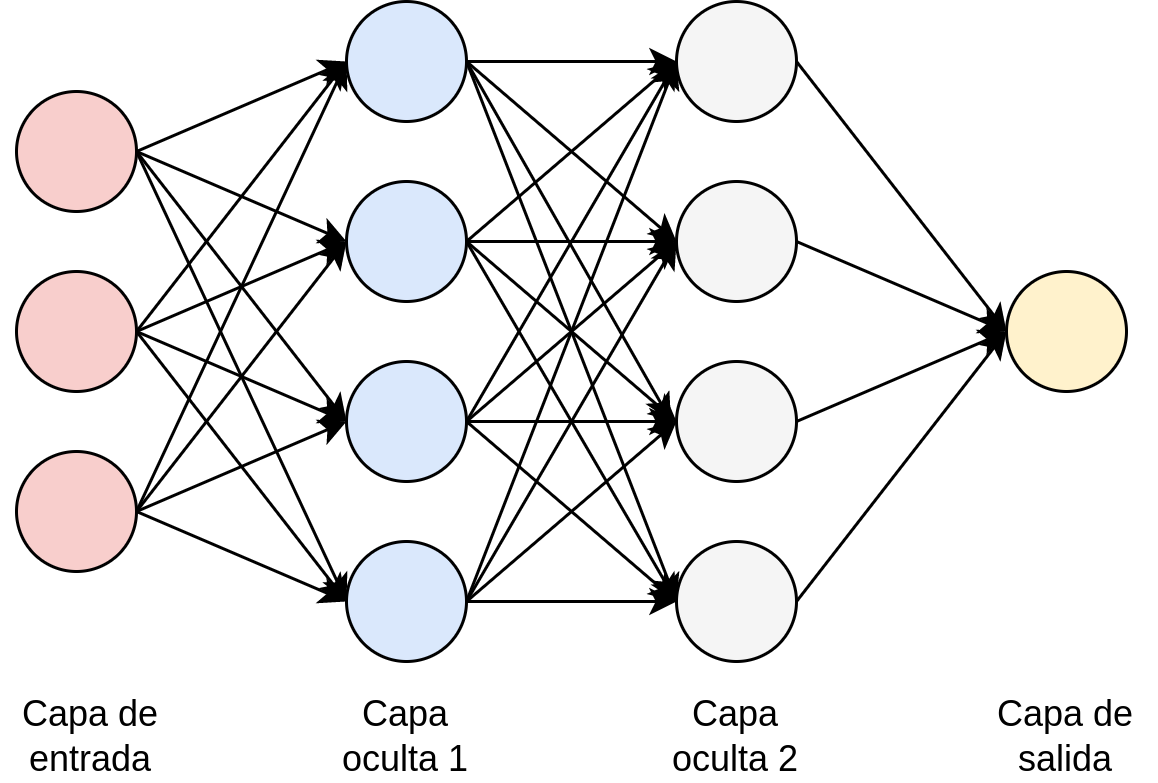
\includegraphics[scale=0.25]{./Figures/dl_nn.png}
	\caption{Arquitectura de una red neuronal artificial.}
	\label{fig:dl_nn}
\end{figure}


Cada uno de los nodos de las capas ocultas y de salida, tienen como entrada la salida de los nodos anteriores multiplicadas por unos términos denominados pesos o \textit{weights} y que sumados junto a otro término llamado sesgo o \textit{bias} pasan por una función de activación no lineal para generar su salida. En la figura \ref{fig:dl_node} se visualiza un nodo de las capas ocultas o de salida.
\begin{figure}[h]
	\centering
	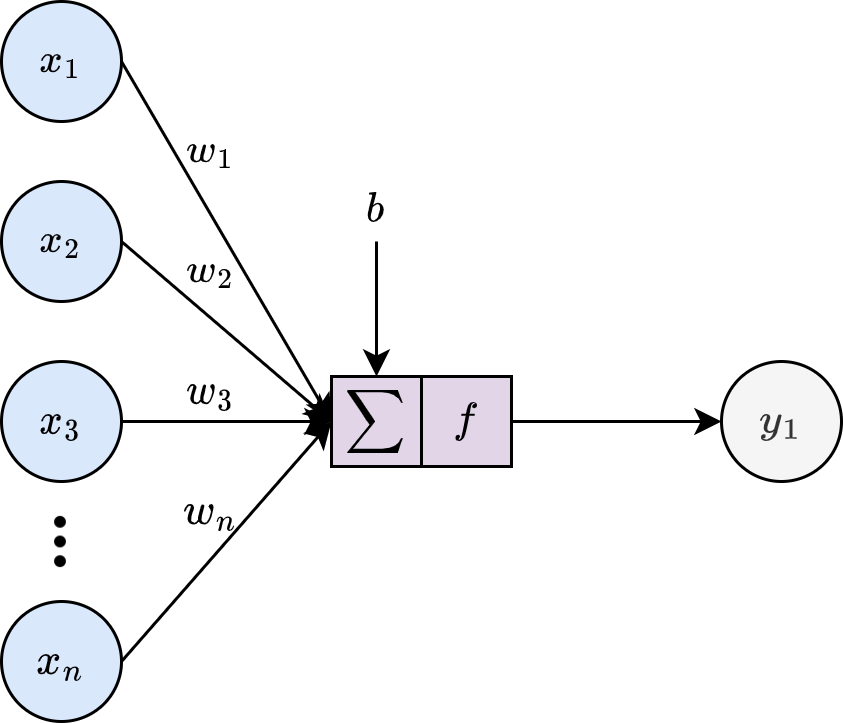
\includegraphics[scale=0.25]{./Figures/dl_node.png}
	\caption{Nodo de una red neuronal artificial.}
	\label{fig:dl_node}
\end{figure}

%----------------------------------------------------------------------------------------
\section{Redes neuronales convolucionales}
También conocidas como CNN (\textit{Convolutional Neural Networks}) por sus siglas en inglés, son un algoritmo de DL que están orientadas a recibir como entrada una imagen digitalizada, asignarle \textit{weights} y \textit{biases} entrenables a varios aspectos/objetos en la imagen para poder diferenciarlas unas de otras \cite{cnn_def}. Su uso reduce el preprocesamiento de las imágenes de entrada con respecto a otros modelos de clasificación, ya que los filtros necesarios son incorporados en su arquitectura y tienen la habilidad de ser entrenados.

Computacionalmente una imagen puede ser muy difícil de procesar, esto depende del espacio de colores donde se encuentra \cite{cnn_colors} y las dimensiones que posee. Por ejemplo, una imagen RGB y de dimensiones 1920x1080 píxeles tiene un tamaño de 6220800 bytes. El objetivo principal de las CNN es reducir la dimensionalidad de las imágenes de entrada, de tal forma que sean más fáciles de procesar y no pierdan sus características o \textit{features} principales que son críticas para obtener una buena predicción.

La arquitectura de una CNN es independiente del tipo de aplicación, donde las capas que lo componen son elegidas en función de los objetivos que se persiguen. En la figura \ref{fig:cnn_arch} se puede observar la arquitectura de una CNN para clasificar dígitos escritos a mano.

\begin{figure}[h]
	\centering
	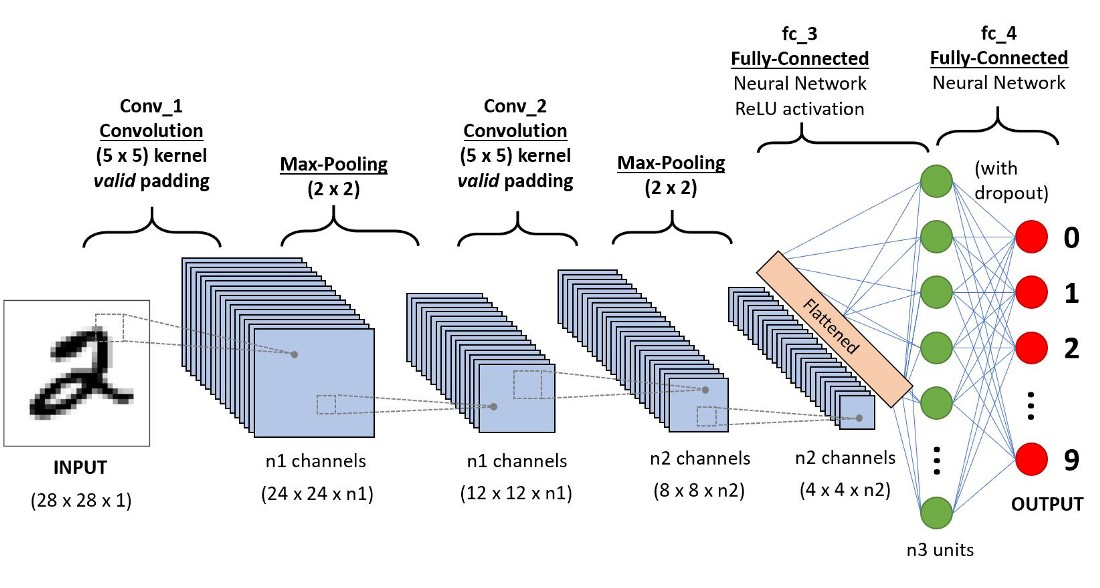
\includegraphics[scale=0.35]{./Figures/cnn_arch.jpeg}
	\caption{CNN para clasificar dígitos escritos a mano\protect\footnotemark.}
	\label{fig:cnn_arch}
\end{figure}
\footnotetext{Imagen tomada de: \url{https://towardsdatascience.com/a-comprehensive-guide-to-convolutional\\-neural-networks-the-eli5-way-3bd2b1164a53}}

En la arquitectura de la figura \ref{fig:cnn_arch} se pueden observar tres capas principales para construir una CNN: capa de convoluciones, capa de \textit{pooling} y capa \textit{fully-connected}.

\subsection{Capa de convoluciones}
Esta capa es la encargada de aplicar la operación de convolución sobre las imágenes de entrada para encontrar patrones que más adelante permitirán clasificarlas. La convolución de una imagen con un \textit{kernel} no es más que la aplicación del operador punto entre ambos. Este tipo de capas se definen por:
\begin{itemize}
	\item El número de los \textit{kernels} o filtros que se aplican a la imagen, que es el número de matrices por las que se van a convolucionar las imágenes de entrada.
	\item El tamaño de los \textit{kernels}, donde casi siempre tienen dimensiones cuadradas e impares como 3x3 o 5x5.
	\item El \textit{stride} o paso, se refiere a la forma en como el \textit{kernel} recorre la imagen.
\end{itemize}

En la figura \ref{fig:cnn_conv} se puede observar la operación de convolución de una entrada con dimensiones 3x3 y un \textit{kernel} de 2x2.

\begin{figure}[h]
	\centering
	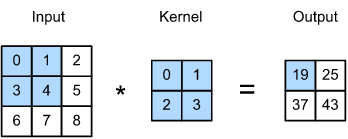
\includegraphics[scale=0.7]{./Figures/cnn_conv.png}
	\caption{Convolución de una entrada de 3x3 con un \textit{kernel} de 2x2 y \textit{stride} de 1\protect\footnotemark.}
	\label{fig:cnn_conv}
\end{figure}
\footnotetext{Imagen tomada de: \url{https://towardsdatascience.com/a-comprehensive-guide-to-convolutional\\-neural-networks-the-eli5-way-3bd2b1164a53}}

\subsection{Capa de \textit{pooling}}
Similar a la capa de convoluciones, tiene el objetivo de reducir la dimensionalidad de los \textit{features} obtenidos mediante las convoluciones aplicadas en la capa anterior, para reducir el poder computacional requerido en un principio. Existen dos tipos de dos tipos: \textit{max pooling} y \textit{Average pooling}. El primero retorna el valor máximo de una porción de la imagen cubierta por el \textit{kernel} y el segundo el valor promedio o \textit{average}. \textit{Max pooling} también funciona como supresor de ruido al mismo tiempo que reduce la dimensionalidad. Mientras que \textit{average pooling} solo sirve para reducir la dimensionalidad. En la figura \ref{fig:cnn_pool} se pueden observar estos tipos de \textit{pooling}.

\begin{figure}[h]
	\centering
	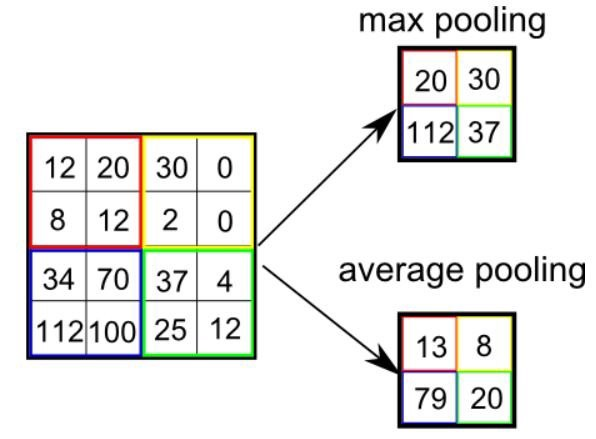
\includegraphics[scale=0.3]{./Figures/cnn_pool.png}
	\caption{Tipos de \textit{pooling}\protect\footnotemark.}
	\label{fig:cnn_pool}
\end{figure}
\footnotetext{Imagen tomada de: \url{https://towardsdatascience.com/a-comprehensive-guide-to-convolutional\\-neural-networks-the-eli5-way-3bd2b1164a53}}

\subsection{Capa \textit{fully-connected}}
También conocida como capa lineal o FC por sus siglas en inglés, es simplemente una red neuronal artificial como la mostrada en la sección anterior y se utiliza después de que las capas de convolución y \textit{pooling} desglosan los \textit{features} más importantes presentes en la imagen de entrada de la CNN. La capa FC brinda las probabilidades finales para cada \textit{label} esperado.

%----------------------------------------------------------------------------------------
\section{Vision artificial}
La visión artificial o \textit{computer vision} es un campo científico interdisciplinario que se encarga de cómo los sistemas computacionales pueden obtener un entendimiento de alto nivel de imágenes y videos digitales para comprender y automatizar tareas como lo haría un sistema de visión humano. Las tareas que ejecuta un sistema de visión artificial son de adquisición, procesamiento, análisis y entendimiento de imágenes. En la figura \ref{fig:mv_comp} se pueden apreciar las similitudes de un sistema de visión artificial y un sistema de visión humano.

\begin{figure}[h]
	\centering
	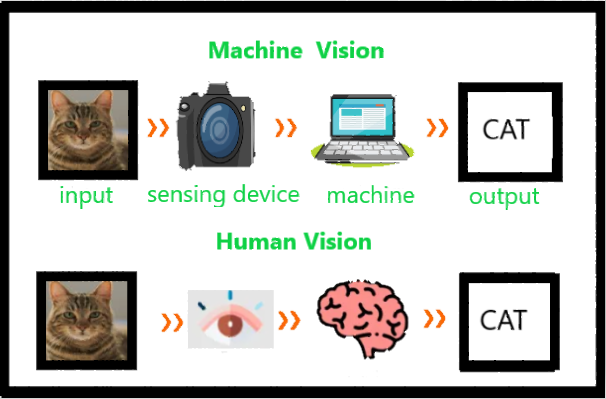
\includegraphics[scale=0.3]{./Figures/mv_comp.png}
	\caption{Componentes de un sistema de visión artificial y un sistema de visión humano.}
	\label{fig:mv_comp}
\end{figure}

Uno de los campos de estudio más importantes de la visión artificial es la detección facial. La detección facial puede ser considerada como un caso particular de la detección de objetos y tiene los objetivos de detectar y localizar todos los rostros humanos contenidos en una imagen digital. En la figura \ref{fig:mv_fd} se puede observar una imagen procesada por un sistema de detección facial.

\begin{figure}[h]
	\centering
	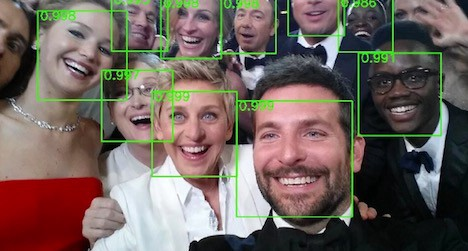
\includegraphics[scale=0.5]{./Figures/mv_fd.jpeg}
	\caption{Imagen procesada por un sistema de detección facial\protect\footnotemark.}
	\label{fig:mv_fd}
\end{figure}
\footnotetext{Imagen tomada de: \url{https://pbarasia.medium.com/use-face-recognition-on-whatsapp-group-\\pictures-part-1-832c6a74b5e5}}

Hoy en día, muchos dispositivos comerciales y profesionales como \textit{smartphones}, \textit{tablets} y robots, utilizan la detección facial como primer paso para otro tipo de aplicaciones más complejas, entre las que destacan: reconocimiento facial, computación afectiva y grabación de vídeo inteligente \cite{fd_apps}.

%----------------------------------------------------------------------------------------
\section{Servicios en la nube}
El término servicios en la nube hace referencia a un amplio rango de servicios ofrecidos bajo demanda a compañías y usuarios a través de internet. Estos servicios están diseñados para proveer de una manera fácil y asequible acceso a aplicaciones y recursos, sin la necesidad de una infraestructura o hardware propios \cite{cs_def}.

Los servicios en la nube son administrados totalmente por proveedores de computación en la nube o \textit{cloud computing} \cite{cs_def}. Estos se encuentran disponibles para los usuarios desde los servidores de los proveedores, por lo que no es necesario que una empresa aloje aplicaciones en sus propios servidores. De manera general, existen tres tipos básicos de servicios en la nube: Software como un servicio (SaaS, \textit{Software as a Service}), Infraestructura como un servicio (IaaS, \textit{Infrastructure as a Service}) y Plataforma como un servicio (PaaS, \textit{Platform as a Service}).

\subsection{Software como un servicio}
En este servicio el proveedor solo proporciona el software o aplicaciones en la nube mediante internet. Los clientes tienen acceso a través de interfaces de aplicación o a través de la web, que les permite interactuar de manera sencilla, sin la necesidad de gestionar, instalar ni actualizar el software.

\subsection{Infraestructura como un servicio}
Este servicio implica la contratación de una infraestructura de hardware a un tercero, donde varios clientes comparten los recursos de una máquina física. El proveedor proporciona a sus clientes el acceso a los recursos computacionales necesarios para almacenar o ejecutar tareas que pueden incluir servidores, redes, \textit{backup}, \textit{firewalls}, entre otros.

\subsection{Plataforma como un servicio}
Es un servicio que se encuentra conceptualmente entre SaaS e IaaS al eliminar la parte física de la infraestructura y ofrece una plataforma donde los clientes pueden crear, desarrollar, gestionar y distribuir sus aplicaciones. El proveedor es el encargado de la gestión y mantenimiento de la plataforma y permite que los clientes se dediquen exclusivamente al desarrollo.

%----------------------------------------------------------------------------------------
\section{Motivación}
Gracias a la amplia gama de plataformas de hardware y la disponibilidad de bibliotecas de código abierto para implementar AI, ML y DL, además de la difusión de información en foros y sitios web especializados, es posible desarrollar sistemas de visión artificial personalizados para distintos tipos de arquitecturas \cite{mot_emb}.

Normalmente las bibliotecas de código y los algoritmos para visión artificial no son aptos para dispostivos con poca cantidad de memoria y poder de computo reducido. Aunque gracias a los constantes avances en el desarrollo de herramientas para optmizar modelos de DL y arquitecturas de modelos mas eficientes y ligeras, es posible implementar estos algoritmos en dispositivos como microcontroladores.

La motivación principal de este trabajo fue desarrollar un sistema embebido de bajo costo económico, bajo consumo energético y de código abierto, que integre algoritmos de DL para visión artificial enfocados en cumplir eficientemente la tarea de detección facial.

Una motivación adicional fue integrar otra tecnología actual como es el internet de las cosas (IoT, \textit{Internet of Things}), para trabajar en conjunto con los algoritmos de visión artificial. Así las aplicaciones que se pueden obtener son más versátiles a la hora de su implementación en entornos urbanos.

%----------------------------------------------------------------------------------------
\section{Estado del arte}
Como antecedente existe el trabajo de Ilhan Aydin y Nashwan Adnan Othman, denominado ``A new IoT combined face detection of people by using computer vision for security application`` \cite{soa_ref}. El \textit{paper} donde se describe su trabajo presenta el desarrollo de un dispositivo electrónico que tiene como componentes principales una Raspberry Pi 3, un sensor pasivo infrarrojo (PIR, \textit{Passive Infra Red}) y una cámara. Su objetivo principal es detectar personas con ayuda del sensor de movimiento PIR, fotografiarlas y aplicar el algoritmo de detección facial Haar Cascade \cite{haar_cascade}, para posteriormente guardar una imagen del rostro detectado y visualizarla en un teléfono móvil con ayuda de la aplicación Telegram. En la figura \ref{fig:soa_arch} se puede observar el diagrama en bloques del sistema descrito anteriormente.

\begin{figure}[h]
	\centering
	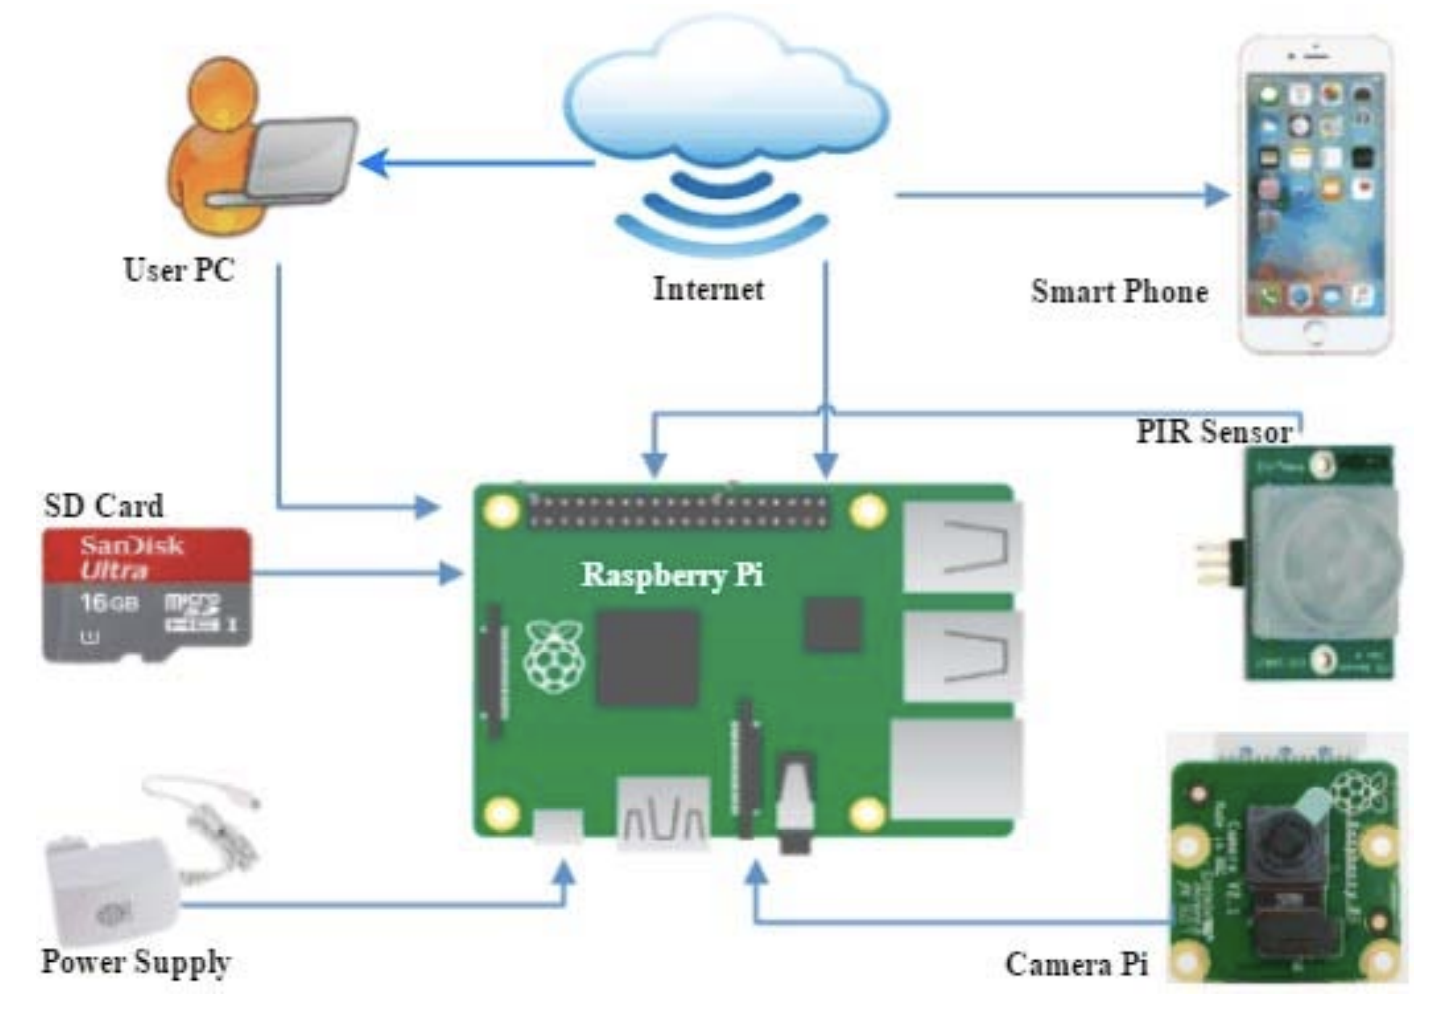
\includegraphics[scale=0.4]{./Figures/soa_arch.png}
	\caption{Diagrama en bloques del sistema propuesto en \cite{soa_ref}}
	\label{fig:soa_arch}
\end{figure}

%----------------------------------------------------------------------------------------
\section{Objetivos y alcance}
El objetivo principal de este trabajo fue desarrollar un sistema embebido con la capacidad de ejecutar modelos de AI para detectar y localizar rostros humanos de imágenes digitales capturadas por su cámara.

El alcance de este trabajo incluyó:
\begin{itemize}
	\item Contruir un prototipo de pruebas
	\item Desarrollar e implementar los modelos de AI necesarios
	\item Implementar los servicios en la nube necesarios
\end{itemize}
%----------------------------------------------------------------------------------------
\section{Requerimientos}
Los requerimientos planteados para este trabajo fueron:
\begin{enumerate}
	\item Requerimientos funcionales
  \begin{enumerate}
     	\item El sistema debe detectar y contar todos los rostros existentes de las imágenes obtenidas por su cámara con ayuda de las técnicas de procesamiento de imágenes \textit{pyramid image} y \textit{slidding window}, y modelos de DL que alcancen una precisión de al menos 80\%.
		\item El sistema debe conectarse a una red Wi-Fi existente a través de algún mecanismo de aprovisionamiento de credenciales de red.
		\item El sistema debe establecer comunicación con los servidores de AWS.
		\item El sistema debe ser alimentado mediante dos baterías AA de litio.
		\item El sistema debe poseer mecanismos de seguridad implementados tanto en hardware como en firmware para evitar su manipulación incorrecta.
		\item El sistema debe funcionar solamente si se detecta movimiento en el sector donde se encuentra instalado.
	\end{enumerate}
	\item Requerimientos no funcionales
	\begin{enumerate}
		\item El sistema debe tener un costo de desarrollo igual o menor a US\$200.
		\item El sistema debe tener documentación adecuada sobre su uso y desarrollo.
	\end{enumerate}
\end{enumerate}



%----------------------------------------------------------------------------------------




